\section{Results}
\label{sec:results}

\para{Overall accuracy is above random but below memorization.}
Across all graph types and context lengths, \directprompt reaches 72.7\% accuracy and \reasonprompt reaches 73.9\%. The deterministic \observedbaseline baseline reaches 82.5\%. Every graph/context cell is above the 50\% random baseline after Holm correction, with corrected $p \leq 0.0328$. However, no cell shows a significant model advantage over \observedbaseline, and \observedbaseline is significantly better in 10 of 20 model-vs-baseline comparisons.

\begin{figure}[t]
    \centering
    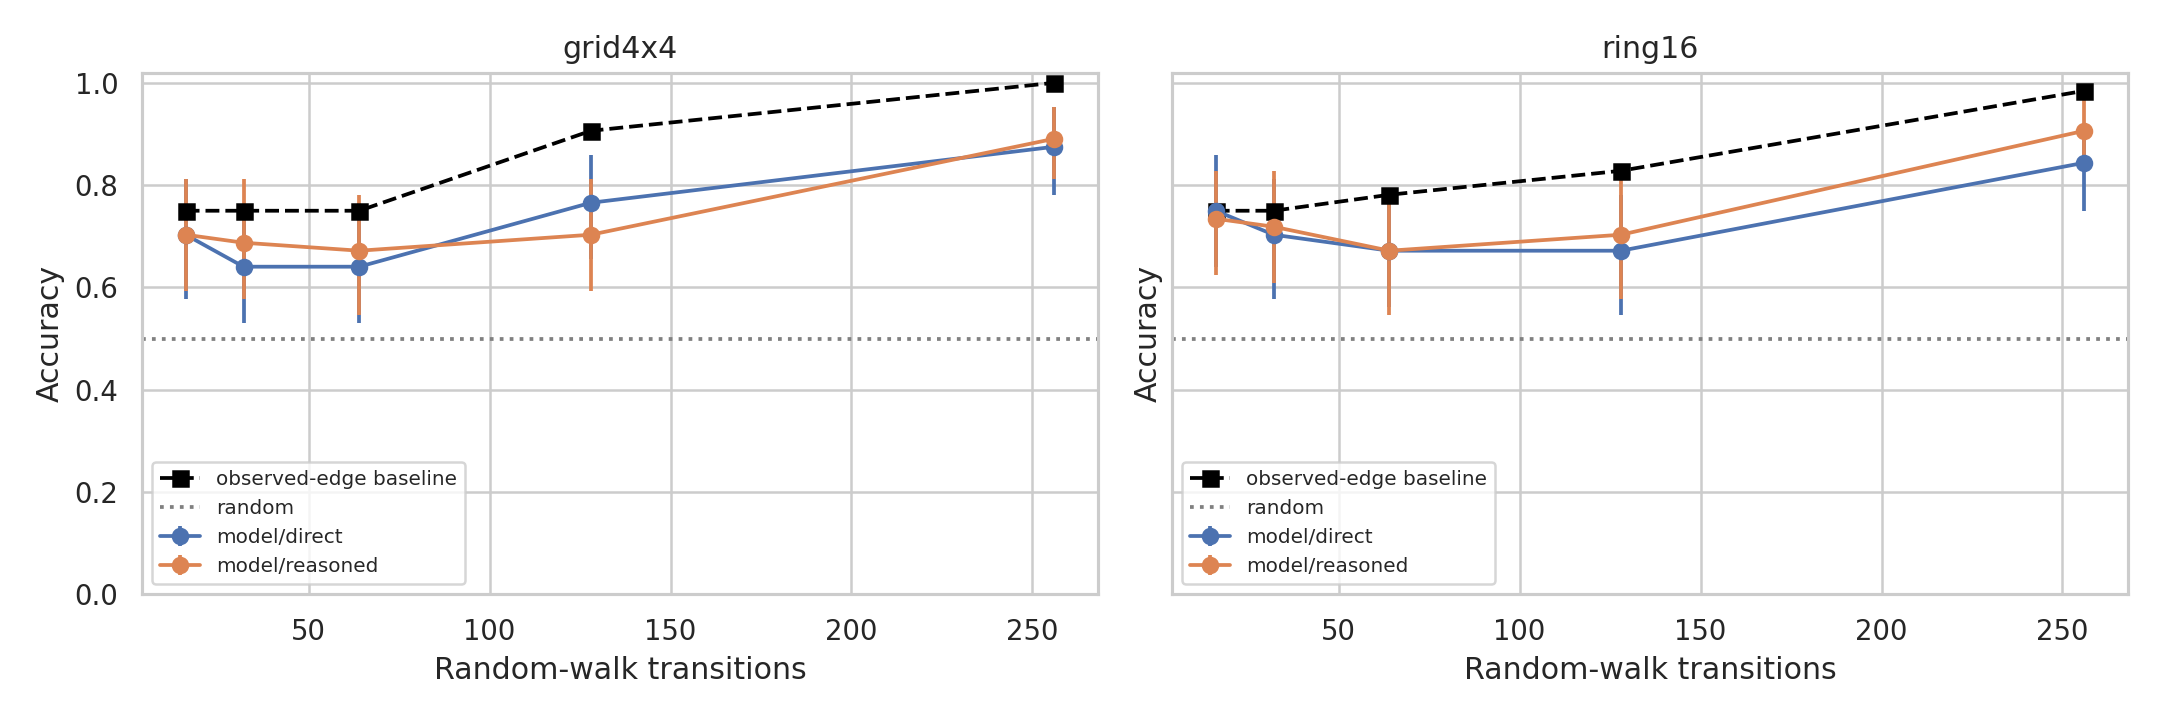
\includegraphics[width=0.95\linewidth]{figures/accuracy_by_context.png}
    \caption{Accuracy by context length. Model accuracy rises at the longest traces, but the curve tracks repeated edge exposure and remains below the observed-edge memorization baseline. Each model point aggregates 64 query-level decisions per graph/context/prompt cell.}
    \label{fig:accuracy_context}
\end{figure}

\begin{table}[t]
    \centering
    \caption{Accuracy by prompt style, graph topology, and context length. Best result for each graph/context setting is in {\bf bold}; ties are both bold. The observed-edge baseline is deterministic and shared across prompt styles.}
    \label{tab:context_accuracy}
    \resizebox{\textwidth}{!}{%
    \begin{tabular}{@{}llccccc@{}}
        \toprule
        \textbf{Prompt} & \textbf{Graph} & \textbf{L=16} & \textbf{L=32} & \textbf{L=64} & \textbf{L=128} & \textbf{L=256} \\
        \midrule
        \directprompt & \gridgraph & 0.703 & 0.641 & 0.641 & 0.766 & 0.875 \\
        \directprompt & \ringgraph & {\bf 0.750} & 0.703 & 0.672 & 0.672 & 0.844 \\
        \reasonprompt & \gridgraph & 0.703 & 0.688 & 0.672 & 0.703 & 0.891 \\
        \reasonprompt & \ringgraph & 0.734 & 0.719 & 0.672 & 0.703 & 0.906 \\
        \observedbaseline & \gridgraph & {\bf 0.750} & {\bf 0.750} & {\bf 0.750} & {\bf 0.906} & {\bf 1.000} \\
        \observedbaseline & \ringgraph & {\bf 0.750} & {\bf 0.750} & {\bf 0.781} & {\bf 0.828} & {\bf 0.984} \\
        \bottomrule
    \end{tabular}
    }
\end{table}


\para{Repeated edges are verbally addressable.}
\Tabref{tab:context_accuracy} shows that longer traces help, especially at $L=256$, where both prompt styles exceed 84\% on both graph families. This gain does not establish topology inference, because the \observedbaseline baseline also rises with trace length and reaches 100.0\% on \gridgraph at $L=256$ and 98.4\% on \ringgraph at $L=256$. The strongest behavioral result is more local: observed true edges are almost perfectly addressable. Both prompt styles answer 158/160 observed-true queries correctly, or 98.8\%.

\begin{figure}[t]
    \centering
    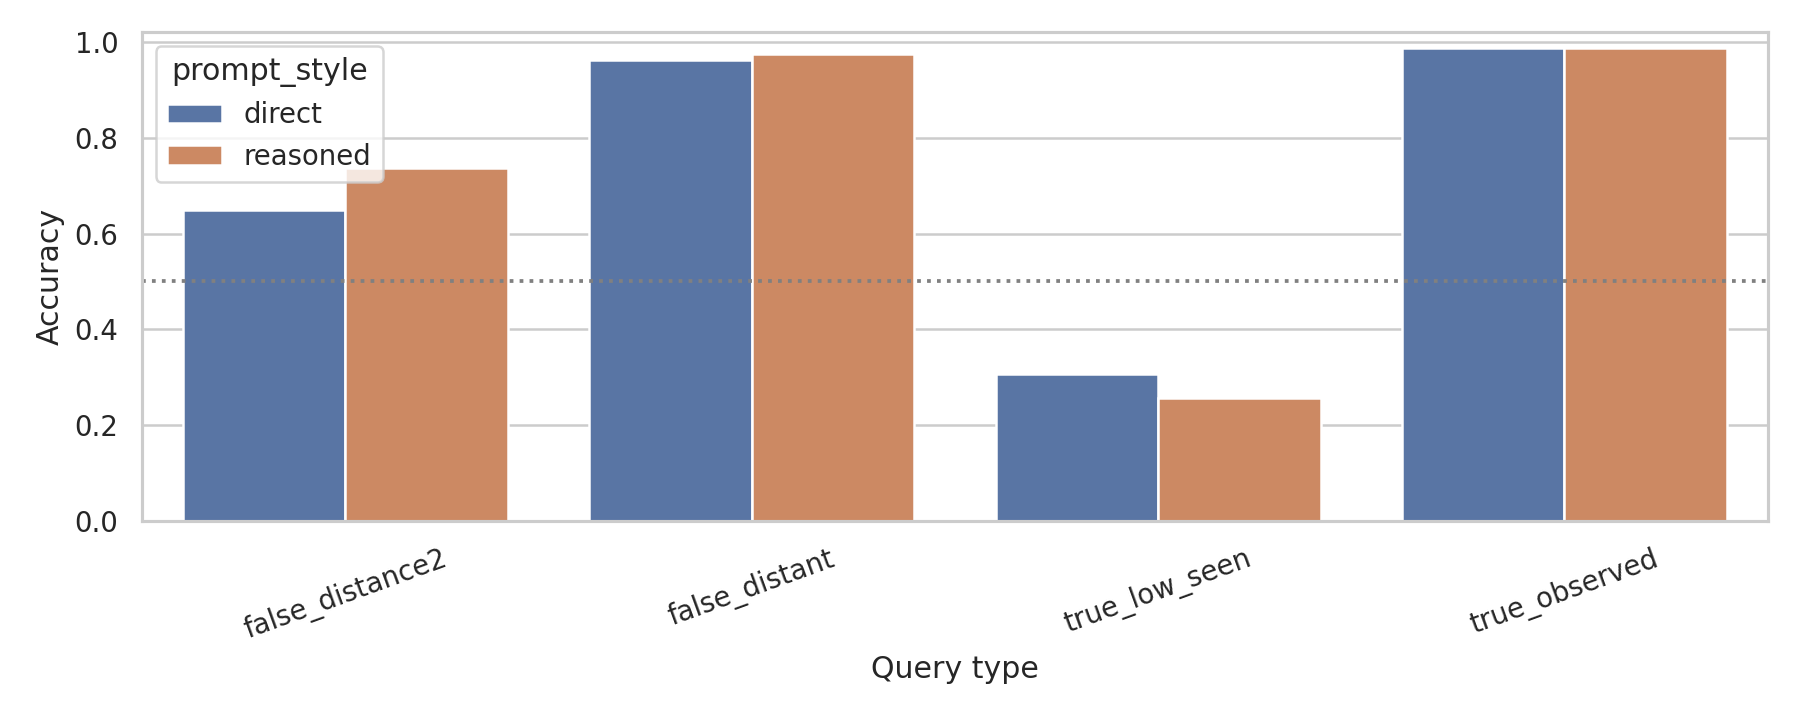
\includegraphics[width=0.9\linewidth]{figures/accuracy_by_query_type.png}
    \caption{Accuracy by query type. Observed true edges are easy, and distant false pairs are mostly rejected. Low-seen true edges are much harder because this category contains many true edges that never appeared in the trace. False distance-2 pairs are also difficult, indicating that the model sometimes treats graph-near words as adjacent.}
    \label{fig:query_type}
\end{figure}

\begin{table}[t]
    \centering
    \caption{Accuracy by query type. Best result in each column is in {\bf bold}. Low-seen true edges include unobserved positives and rare observed positives; the unobserved-only slice is analyzed separately in the text and in \figref{fig:unobserved_true}.}
    \label{tab:query_type_accuracy}
    \resizebox{\textwidth}{!}{%
    \begin{tabular}{@{}lcccc@{}}
        \toprule
        \textbf{Prompt or baseline} & \textbf{Observed true} & \textbf{Low-seen true} & \textbf{False distance-2} & \textbf{False distant} \\
        \midrule
        \directprompt & 0.988 & {\bf 0.306} & 0.650 & 0.963 \\
        \reasonprompt & 0.988 & 0.256 & 0.738 & 0.975 \\
        \observedbaseline & {\bf 1.000} & 0.300 & {\bf 1.000} & {\bf 1.000} \\
        \bottomrule
    \end{tabular}
    }
\end{table}


\para{The critical slice is unobserved true edges.}
The low-seen true category in \tabref{tab:query_type_accuracy} mixes rare observed edges with unobserved edges. When we isolate true edges with observed count zero, the model nearly always says \texttt{NO}. \directprompt recovers only 4/112 unobserved true adjacencies, or 3.6\%. \reasonprompt recovers 0/112. In contrast, once a low-seen true edge appears twice, \directprompt answers all 11 such cases correctly; at three or more observations, both prompt styles are perfect on this slice. The failure is therefore not a general inability to answer \texttt{YES}; it is a failure to infer missing positive edges from sparse topology.

\begin{figure}[t]
    \centering
    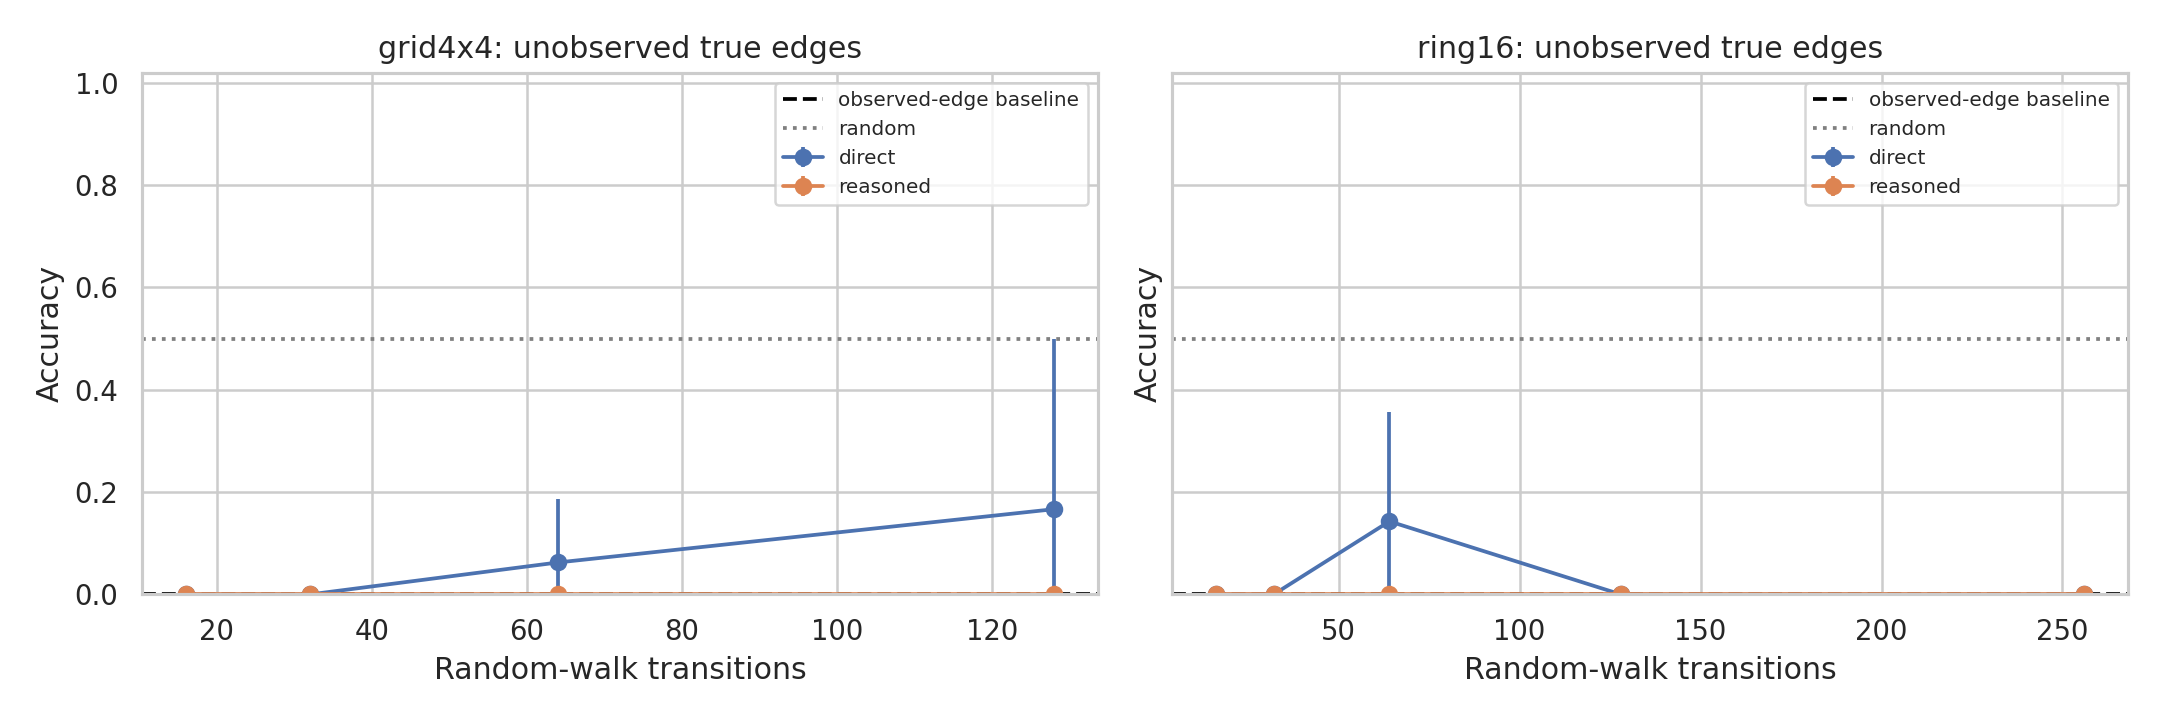
\includegraphics[width=0.95\linewidth]{figures/unobserved_true_edge_accuracy.png}
    \caption{Accuracy on true graph edges that never appeared in the prompt trace. The model rarely recovers these missing positives, even though they are valid adjacencies in the hidden graph. Explicit reasoning does not improve this slice.}
    \label{fig:unobserved_true}
\end{figure}

\para{Explicit reasoning changes errors but does not solve addressability.}
The explicit-reasoning prompt improves overall accuracy by only 1.25 percentage points, from 72.7\% to 73.9\%. A paired direct-vs-reasoned McNemar test is not significant ($p=0.256$). Reasoning helps reject some near false pairs: false distance-2 accuracy increases from 65.0\% to 73.8\%. But this comes with worse positive recovery in the low-seen slice, which drops from 30.6\% to 25.6\%, and with complete failure on unobserved true edges.
